\documentclass{article}
\usepackage[margin=2.54cm]{geometry}
\usepackage{graphicx}   % imágenes
\graphicspath{{img}}
\usepackage{amsfonts}   % fuentes de conjuntos numéricos
\usepackage{amsmath}
\usepackage{tikz}       % gráficos
\usepackage{pgfplots}   % plots
\pgfplotsset{width=10cm, compat=1.9}
\setlength{\jot}{8pt}
\setlength{\parindent}{0cm}
\usepackage{parskip}    % espacio entre párrafos
\usepackage{cancel}     % cancelar términos
\usepackage[colorlinks=true, urlcolor=blue]{hyperref}   % links
\usetikzlibrary{shapes.geometric}   % shapes
\usepackage{pdfpages}   % incluir pdfs

\title{porfolio final}
\author{Daniel Ise}
\date{June 2024}

\begin{document}
\begin{titlepage}
    \begin{center}
        \vspace*{.5cm}
        \includegraphics[scale=.5]{img/udemm-logo.png}\\
        \vspace{.2cm}
        \Large
        \textbf{Facultad de Ingeniería}\\
        \textbf{Ingeniería en Sistemas}\\
        \vspace{2cm}

        \Huge
        Análisis de Sistemas II \\
        Examen Parcial I \\
        Iteración N\(^\circ\) 2 \\
        \vfill

        \raggedright
        \Large
        Docentes:
        \begin{itemize}
            \item[] Mg. Margarita Castronuovo \\
        \end{itemize}
        Alumno:
        \begin{itemize}
            \item[] Daniel Ise
        \end{itemize}
        Legajo:
        \begin{itemize}
            \item[] 28547
        \end{itemize}
        Fecha:
        \begin{itemize}
            \item[] Mayo, 2025
        \end{itemize}
    \end{center}
\end{titlepage}

\section*{Unidad 1: Números reales}

\subsection*{Actividad 1.A}
\textbf{Deducir y demostrar geométricamente, a partir de dos cuadrados
	de lado “a” y “b”, respectivamente, y otros dos rectángulos de largo
	“a” y ancho “b” que $(a + b)^2 = a^2 + 2ab + b^2$.}

Dado un cuadrado de lado $a$, con $a \in \mathbb{R^+}$, podemos definir su área como $a^2$.

\begin{center}
	\begin{tikzpicture}
		\draw[blue] (0,0) rectangle (2,2);
		\draw (1, -0.4) node{$a$};
	\end{tikzpicture}
\end{center}

De igual manera, podemos definir un cuadrado de lado $b$, con $b \in \mathbb{R^+}$, siendo su área $b^2$.

\begin{align*}
	\begin{tikzpicture}
		\draw[red] (0,0) rectangle (1.5,1.5);
		\draw (.75, -0.4) node{$b$};
	\end{tikzpicture}
\end{align*}

Entonces, si definimos un tercer cuadrado, de lado $a+b$, su área vendría dada por la expresión $(a+b)^2$. Gráficamente:

\begin{align*}
	\begin{tikzpicture}
		% Cuadrado a
		\draw[blue] (0,0) -- (2,0);
		\draw[blue] (0,0) -- (0,2);
		\draw[blue,dashed] (2,0) -- (2,2);
		\draw[blue,dashed] (0,2) -- (2,2);
		\draw (1, -0.4) node{$a$};
		% Cuadrado b
		\draw[red,dashed] (2,2) -- (3.5,2);
		\draw[red,dashed] (2,2) -- (2,3.5);
		\draw[red] (3.5,2) -- (3.5,3.5);
		\draw[red] (2,3.5) -- (3.5,3.5);
		\draw (3.9, 2.75) node{$b$};
		% Resto
		\draw[red] (2,0) -- (3.5,0);
		\draw (2.75, -0.4) node{$b$};
		\draw[blue] (3.5, 0) -- (3.5, 2);
		\draw (3.9, 1) node{$a$};
		\draw[blue] (0, 3.5) -- (2, 3.5);
		\draw (1, 3.9) node{$a$};
		\draw[red] (0, 2) -- (0, 3.5);
		\draw (-0.4, 2.75) node{$b$};
		\draw (2.75, 3.9) node{$b$};
		\draw (-0.4, 1) node{$a$};
	\end{tikzpicture}
\end{align*}

Como vemos, el cuadrado resultante es la sumatoria de las áreas de los cuadrados 1 y 2, más dos rectángulos de área $a \cdot b$. Por lo cual el área de un cuadrado de lado $a+b$ es igual a $a^2 + ab + ab + b^2$, es decir, $(a + b)^2 = a^2 + 2ab + b^2$.

\subsection*{Actividad 1.B}
\textbf{A partir de la deducción anterior, interpretar en forma gráfica la expresión: $x^2 + 4x + 4$}

La expresión $x^2 + 4x + 4$ se puede interpretar gráficamente como un cuadrado de lado $x + 2$.

\begin{align*}
\begin{tikzpicture}
	% Cuadrado a
\draw[cyan] (0,0) -- (2,0);
\draw[cyan] (0,0) -- (0,2);
\draw[cyan,dashed] (2,0) -- (2,2);
\draw[cyan,dashed] (0,2) -- (2,2);
\draw (1, -0.4) node{$x$};
\draw (-0.4, 1) node{$x$};
	% Cuadrado b
\draw[orange,dashed] (2,2) -- (3.5,2);
\draw[orange,dashed] (2,2) -- (2,3.5);
\draw[orange] (3.5,2) -- (3.5,3.5);
\draw[orange] (2,3.5) -- (3.5,3.5);
\draw (3.9, 2.75) node{$2$};
\draw (2.75, 3.9) node{$2$};
	% Resto
\draw[orange] (2,0) -- (3.5,0);
\draw (2.75, -0.4) node{$2$};
\draw[cyan] (3.5, 0) -- (3.5, 2);
\draw (3.9, 1) node{$x$};
\draw[cyan] (0, 3.5) -- (2, 3.5);
\draw (1, 3.9) node{$x$};
\draw[orange] (0, 2) -- (0, 3.5);
\draw (-0.4, 2.75) node{$2$};
\end{tikzpicture}
\end{align*}

De esta forma, si sumamos las áreas de los cuadrados y rectángulos que componen al cuadrado de lado $(x+2)$ obtenemos que $(x+2)^2 = x^2 + 2x + 2x + 2^2$, que puede expresarse como $x^2 + 4x +4$.

\subsection*{Actividad 1.C}
\textbf{Consigna. }
Proponer una deducción de la fórmula Bhaskara o \textit{resolvente},
empleada en la resolución de ecuaciones cuadráticas.

Dados $a, b, c \in \mathbb{R}$, con $a \neq 0$,
una expresión cuadrática puede definirse como el polinomio de estructura $ax^2 + bx + c = 0$,
siendo $a$ el coeficiente cuadrático,
$b$ el coeficiente lineal
y $c$ el término independiente.

Para deducir Bhaskara desde esta expresión empleamos la técnica de completar el cuadrado.
En primer lugar,
dividimos todos los términos por $a$,
para asegurar que el coeficiente lineal es igual a 1:

\begin{align*}
	\frac{ax^2}{a} + \frac{bx}{a} + \frac{c}{a} & = \frac{0}{a} \\
\end{align*}

Despejamos el término independiente:

\begin{align*}
	x^2 + \frac{bx}{a} & = \frac{-c}{a} \\
\end{align*}

Para completar el cuadrado buscamos la estructura $x^2 + 2nx + n^2$,
por lo que multiplicamos al término lineal por $\frac{2}{2}$:

\begin{align*}
	x^2 + \frac{2}{2} \cdot \frac{bx}{a} & = - \frac{c}{a} \\
	x^2 + 2 \cdot \frac{b}{2a} \cdot x   & = - \frac{c}{a} \\
\end{align*}

Como $2 \cdot \frac{b}{2a} \cdot x$ sigue la estructura $2nx$, sumamos $n^2$ a ambos lados:

\begin{align*}
	x^2 + 2 \cdot \frac{b}{2a} \cdot x + \left(\frac{b}{2a}\right)^2 & = \left(\frac{b}{2a}\right)^2 - \frac{c}{a} \\
\end{align*}

Expresamos la componente izquierda como un binomio al cuadrado y del lado derecho operamos la resta de fracciones:

\begin{align*}
	\left(x + \frac{b}{2a}\right)^2 & = \frac{b^2 - 4ac}{4a^2} \\
\end{align*}

Operamos raíz cuadrada a ambos lados de la expresión, incorporando módulo del lado izquierdo.

\begin{align*}
	\left|x + \frac{b}{2a}\right| & = \sqrt{\frac{b^2 - 4ac}{4a^2}} \\
	\left|x + \frac{b}{2a}\right| & = \frac{\sqrt{b^2 - 4ac}}{\sqrt{4a^2}} \\
	\left|x + \frac{b}{2a}\right| & = \frac{\sqrt{b^2 - 4ac}}{2a}
\end{align*}

En este punto diversificamos, una expresión para cuando \(x + \frac{b}{2a} \geq 0\):

\begin{align*}
	x + \frac{b}{2a} & = \frac{\sqrt{b^2 - 4ac}}{2a} \\
	x  & =  - \frac{b}{2a} + \frac{\sqrt{b^2 - 4ac}}{2a} \\
	x  & =  \frac{-b + \sqrt{b^2 - 4ac}}{2a} \\
\end{align*}

Y otra para \(x + \frac{b}{2a} < 0\):

\begin{align*}
	- x - \frac{b}{2a} & = \frac{\sqrt{b^2 - 4ac}}{2a} \\
	- x  & = \frac{b}{2a} + \frac{\sqrt{b^2 - 4ac}}{2a} \\
	x  & =  \frac{-b - \sqrt{b^2 - 4ac}}{2a} \\
\end{align*}

Estas dos expresiones se unifican en la conocida fórmula Bhaskara:

\begin{align*}
	x & = \frac{-b \pm \sqrt{b^2 - 4ac}}{2a} \\
\end{align*}

\subsection*{Actividad 1.D}
\textbf{Una inecuación es una desigualdad entre dos expresiones
	algebraicas con una o varias incógnitas.
	Los coeficientes de la x también pueden pasar al otro lado como en
	las ecuaciones, pero tenemos que cambiar el signo de
	desigualdad si el número es negativo. ¿Por qué?}

Dados tres números $a, b, x \in \mathbb{R}$, una inecuación puede expresarse como:

\begin{align*}
	ax & \leq b \\
\end{align*}

Dado un número $n \in \mathbb{R}$, sumar o restar $n$ a ambos miembros de la expresión mantiene la desigualdad:

\begin{align*}
	-2     & < 1     \\
	-2 - 1 & < 1 - 1 \\
	-3     & < -2
\end{align*}

La situación puede cambiar cuando operamos productos a ambos lados de la desigualdad.

\begin{align*}
	-2         & < 1         \\
	-2 \cdot 2 & < 1 \cdot 2 \\
	-4         & < 2
\end{align*}

Como vemos, la inecuación se sigue verificando para este producto, siendo ese el caso para todo $n \in \mathbb{R^+}$. Sin embargo, la situación cambia al multiplicar números negativos.

\begin{align*}
	-2 \cdot -2 & \not < 1 \cdot -2 \\
	4           & \not < -2         \\
	4           & > -2
\end{align*}

Al multiplicar ambos miembros de una inecuación por un número $n \in \mathbb{R^-}$, es necesario cambiar la orientación de la desigualdad, de manera tal que esta se siga verificando.

\subsection*{Actividad 2}
\textbf{Consigna.}
Proponer y resolver en forma algebraica y gráfica una situación
problemática relacionada con su carrera de grado que se resuelva a
partir de un sistema de ecuaciones de dos ecuaciones lineales con
dos incógnitas, cuyo resultado sea el par ordenado S=(a, b) siendo
“a” el primer número de su documento y “b” , el último número del
mismo.

Tenemos un servicio en línea dedicado a validar identidades para evitar el fraude en ventas por internet. El principal costo del servicio es el pago al proveedor de computación en la nube, cuyo precio final se compone de un monto fijo mensual, más un costo variable que depende de la cantidad de validaciones que se hagan en el mes. El costo total sigue el modelo $c = 2 + \frac{2}{3} \cdot v$, siendo $2$ el costo fijo, $v$ la cantidad de validaciones medidas en miles y $c$ el costo total en dólares.

Si el precio competitivo para nuestro servicio es de \$ 0,00133 por validación ¿Cuál es la cantidad mínima de validaciones necesarias para que el servicio sea rentable?

En primer lugar, planteamos un modelo para los ingresos, expresando el precio en miles: $i = \frac{4}{3} \cdot v$.

El servicio sería rentable si cubrimos, como mínimo, la totalidad de los costos, por lo tanto:

\begin{align*}
    i - c                                                       & = 0 \\
    \frac{4}{3} \cdot v - \left(2 + \frac{2}{3} \cdot v \right) & = 0 \\
    \frac{2}{3} \cdot v                                         & = 2 \\
    v                                                           & = 3
\end{align*}

Entonces, a partir de $v = 3$ (3000 validaciones mensuales) el servicio sería rentable, igualándose costos e ingresos en \$ 4 por mes.

Gráficamente:

\begin{center}
    \begin{tikzpicture}
        \begin{axis}[
                axis lines = left,
                xlabel = \(v\),
                ylabel = {\(\$\)},
                clip = false,
            ]
            % costo
            \addplot [
                domain=0:8,
                samples=200,
                color=cyan,
            ]
            {2 + x*2/3};
            \addlegendentry{\(2 + \frac{2}{3} \cdot v\)}

            % ingreso
            \addplot [
                domain=0:8,
                samples=200,
                color=orange,
            ]
            {x*4/3};
            \addlegendentry{\(\frac{4}{3} \cdot v\)}
            \node[label={270:{(3,4)}},circle,fill,inner sep=2pt] at (axis cs:3,4) {};
        \end{axis}
    \end{tikzpicture}
\end{center}

\href{https://drive.google.com/file/d/1DXpY7xukQlkF4CswWKmvItGMWZuxZohS/view?usp=sharing}{Link para el audio.}


\section*{Unidad 1: Números reales}

\subsection*{Actividad 1.A}
\textbf{Deducir y demostrar geométricamente, a partir de dos cuadrados
	de lado “a” y “b”, respectivamente, y otros dos rectángulos de largo
	“a” y ancho “b” que $(a + b)^2 = a^2 + 2ab + b^2$.}

Dado un cuadrado de lado $a$, con $a \in \mathbb{R^+}$, podemos definir su área como $a^2$.

\begin{center}
	\begin{tikzpicture}
		\draw[blue] (0,0) rectangle (2,2);
		\draw (1, -0.4) node{$a$};
	\end{tikzpicture}
\end{center}

De igual manera, podemos definir un cuadrado de lado $b$, con $b \in \mathbb{R^+}$, siendo su área $b^2$.

\begin{align*}
	\begin{tikzpicture}
		\draw[red] (0,0) rectangle (1.5,1.5);
		\draw (.75, -0.4) node{$b$};
	\end{tikzpicture}
\end{align*}

Entonces, si definimos un tercer cuadrado, de lado $a+b$, su área vendría dada por la expresión $(a+b)^2$. Gráficamente:

\begin{align*}
	\begin{tikzpicture}
		% Cuadrado a
		\draw[blue] (0,0) -- (2,0);
		\draw[blue] (0,0) -- (0,2);
		\draw[blue,dashed] (2,0) -- (2,2);
		\draw[blue,dashed] (0,2) -- (2,2);
		\draw (1, -0.4) node{$a$};
		% Cuadrado b
		\draw[red,dashed] (2,2) -- (3.5,2);
		\draw[red,dashed] (2,2) -- (2,3.5);
		\draw[red] (3.5,2) -- (3.5,3.5);
		\draw[red] (2,3.5) -- (3.5,3.5);
		\draw (3.9, 2.75) node{$b$};
		% Resto
		\draw[red] (2,0) -- (3.5,0);
		\draw (2.75, -0.4) node{$b$};
		\draw[blue] (3.5, 0) -- (3.5, 2);
		\draw (3.9, 1) node{$a$};
		\draw[blue] (0, 3.5) -- (2, 3.5);
		\draw (1, 3.9) node{$a$};
		\draw[red] (0, 2) -- (0, 3.5);
		\draw (-0.4, 2.75) node{$b$};
		\draw (2.75, 3.9) node{$b$};
		\draw (-0.4, 1) node{$a$};
	\end{tikzpicture}
\end{align*}

Como vemos, el cuadrado resultante es la sumatoria de las áreas de los cuadrados 1 y 2, más dos rectángulos de área $a \cdot b$. Por lo cual el área de un cuadrado de lado $a+b$ es igual a $a^2 + ab + ab + b^2$, es decir, $(a + b)^2 = a^2 + 2ab + b^2$.

\subsubsection*{Modelización de dos variables}

Tenemos que construir un silo de forma cilíndrica para el almacenamiento de granos. La capacidad de almacenamiento del silo viene dada por la función $V(r, h)$, que depende de dos variables: radio de la base del silo ($r$) y su altura ($h$).

\begin{center}
    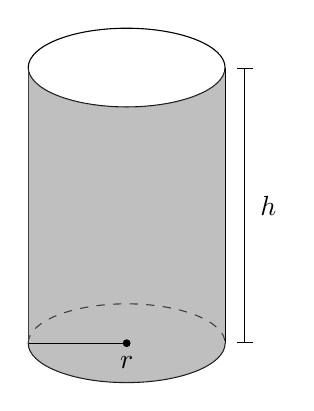
\begin{tikzpicture}
        \draw (0,0) ellipse (1.25 and 0.5);
        \draw (-1.25,0) -- (-1.25,-3.5);
        \draw (-1.25,-3.5) arc (180:360:1.25 and 0.5);
        \draw [dashed] (-1.25,-3.5) arc (180:360:1.25 and -0.5);
        \draw (1.25,-3.5) -- (1.25,0);
        \fill [gray,opacity=0.5] (-1.25,0) -- (-1.25,-3.5) arc (180:360:1.25 and 0.5) -- (1.25,0) arc (0:180:1.25 and -0.5);
        \draw (1.8,-1.75) node{$h$};
        \draw [|-|] (1.5,0) -- (1.5,-3.5);
        \draw (0,-3.75) node{$r$};
        \draw [line width=0.0mm] (-1.24,-3.5) -- (0,-3.5);
        \node at (0,-3.5) [circle,fill,inner sep=1pt]{};
    \end{tikzpicture}
\end{center}

Definimos la función de la capacidad de almacenamiento del silo como:

\begin{align*}
    V(r, h) & = \pi r^2h
\end{align*}

Por motivos estructurales, el radio no puede ser menor a 1 metro y la altura no puede superar los 24 metros. 
A su vez, 
por el material elegido, 
la altura no debe superar 3 veces al radio. 
Por lo tanto:

\begin{align*}
    3r = h
\end{align*}

Sustituimos en la expresión original:

\begin{align*}
    V & = \pi r^2 \cdot 3r \\
    V & = 3 \pi r^3
\end{align*}

Gráficamente:

\begin{center}
    \begin{tikzpicture}
        \begin{axis}[
                axis lines = left,
                xlabel = \(r\),
                ylabel = {\(V\)},
                clip = false,
                legend pos = outer north east,
                ymin = 0,
                xmin = 0,
            ]
            % volumen
            \addplot [
                domain=1:8,
                samples=200,
                color=orange,
            ]
            {3 * 3.14159265 * x * x * x};
            \addlegendentry{\(V = 3 \pi r^3\)}


        \end{axis}
    \end{tikzpicture}
\end{center}

Dadas las restricciones al radio y la altura, el dominio de la función sería $D = [1; 8]$.

Por su parte, la imagen sería $I = [9.43; 4825.49]$.

\subsection*{Actividad 2}

\begin{center}
    Consumo de heladeras en vatios por hora, según eficiencia\\
    \vspace{4mm}
    \begin{tabular}{ccccc}
        Horas & A     & C   & D   & E   \\ \hline
        0     & 0     & 0   & 0   & 0   \\
        1     & 26.5  & 41  & 50  & 59  \\
        2     & 53    & 82  & 100 & 118 \\
        3     & 79.5  & 123 & 150 & 177 \\
        4     & 106   & 164 & 200 & 236 \\
        5     & 132.5 & 205 & 250 & 295 \\
        6     & 159   & 246 & 300 & 354 \\ \hline
        \vspace{5mm}
    \end{tabular}
\end{center}

Gráficamente:

\begin{center}
    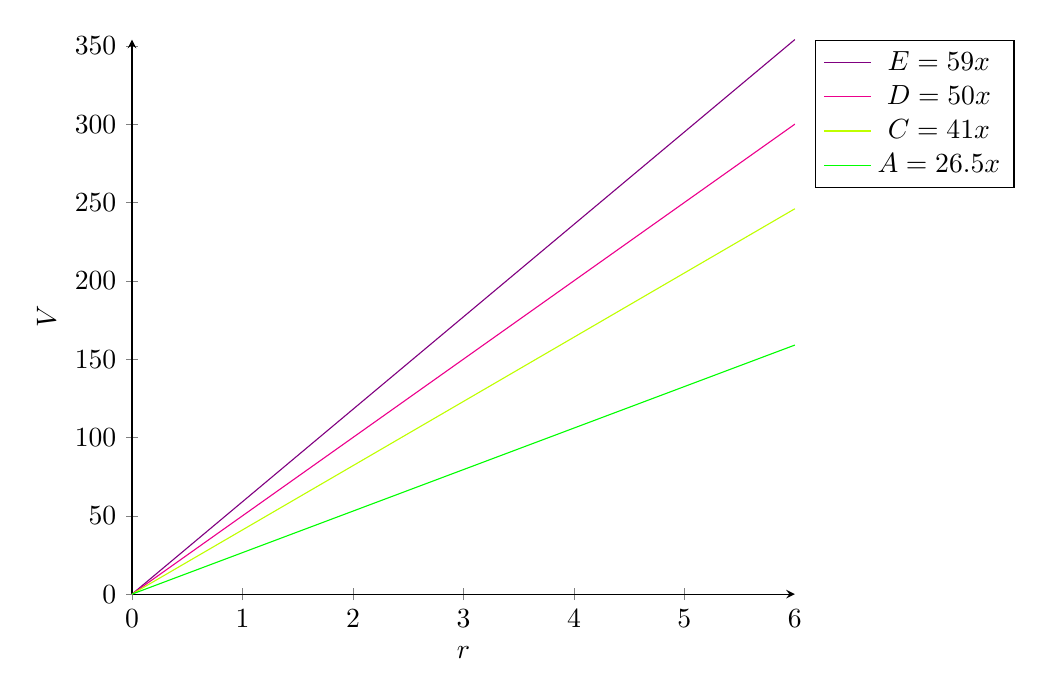
\begin{tikzpicture}
        \begin{axis}[
                axis lines = left,
                xlabel = \(r\),
                ylabel = {\(V\)},
                clip = false,
                legend pos = outer north east,
                ymin = 0,
                xmin = 0,
            ]

            % E
            \addplot [
                domain=0:6,
                samples=200,
                color=violet,
            ]
            {59 * x};
            \addlegendentry{\(E = 59x\)}

            % D
            \addplot [
                domain=0:6,
                samples=200,
                color=magenta,
            ]
            {50 * x};
            \addlegendentry{\(D = 50x\)}

            % C
            \addplot [
                domain=0:6,
                samples=200,
                color=lime,
            ]
            {41 * x};
            \addlegendentry{\(C = 41x\)}

            % A
            \addplot [
                domain=0:6,
                samples=200,
                color=green,
            ]
            {26.5 * x};
            \addlegendentry{\(A = 26.5x\)}

        \end{axis}
    \end{tikzpicture}
\end{center}

Las función de consumo de cada categoría de heladera es:

\begin{align*}
    A(h) & = 26.5h \\
    C(h) & = 41h   \\
    D(h) & = 50h   \\
    E(h) & = 59h
\end{align*}

La pendiente de cada función indica el consumo en vatios por hora de cada categoría de heladera.

Una heladera de eficiencia A consume 636 vatios por día, mientras una heladera de eficiencia E consume 1416 vatios por día. Usar una heladera de tipo A permite ahorrar hasta un 55\% de vatios al día.



\section*{Unidad 3: Límites y continuidad}

\subsection*{Actividad 1}

\textbf{Realizar un mapa conceptual de la unidad, que incluya los
principales conceptos desarrollados.}

\subsection*{Límites}
\begin{center}
	\includegraphics[trim={1.5cm 18.3cm 0 2cm},clip,scale=.84]{03/02mapa-limites.pdf}
\end{center}

\subsection*{Cálculo de Límites}
\begin{center}
	\includegraphics[trim={1.5cm 1.7cm 0 11.6cm},clip,scale=.84]{03/03mapa-calculo-limites.pdf}
\end{center}

\subsection*{Asíntotas}
\begin{center}
	\includegraphics[trim={1.5cm 15cm 0 2cm},clip,scale=.84]{03/04mapa-asintotas.pdf}
\end{center}

\subsection*{Continuidad}
\begin{center}
	\includegraphics[trim={1.5cm 1.7cm 0 14cm},clip,scale=.84]{03/05mapa-continuidad.pdf}
\end{center}

\subsection*{Actividad 2.A}

\begin{center}
\begin{tikzpicture}
\begin{axis}[
    axis lines = center,
    clip = false,
    legend pos = outer north east,
]
% x < -2
\addplot [
    domain=-4:-2, 
    samples=100, 
    color=magenta,
]
{x-1};

% x = -2
\node[circle,fill,inner sep=2pt, color=magenta] at (axis cs:-2,1) {};

% x > -2
\addplot [
    domain=-2:-1, 
    samples=100, 
    color=magenta,
]
{x};

% x > -1
\addplot [
    domain=-1:4, 
    samples=100, 
    color=magenta,
]
{(x*x - x)/(x)};

\node[circle,
    fill=white,
    draw,
    outer sep=0pt,
    inner sep=1.5pt] at (axis cs:0,-1) {};

\end{axis}
\end{tikzpicture}
\end{center}

\begin{align*}
    f(x) = 
    \begin{cases}
        x-1, & \text{si } x < -2\\
        1, & \text{si } x = -2\\
        x, & \text{si } -2 < x < -1\\
        \frac{x^2-x}{x}, & \text{si } x \ge -1
    \end{cases}
\end{align*}



\section*{Unidad 1: Números reales}

\subsection*{Actividad 1.A}
\textbf{Deducir y demostrar geométricamente, a partir de dos cuadrados
	de lado “a” y “b”, respectivamente, y otros dos rectángulos de largo
	“a” y ancho “b” que $(a + b)^2 = a^2 + 2ab + b^2$.}

Dado un cuadrado de lado $a$, con $a \in \mathbb{R^+}$, podemos definir su área como $a^2$.

\begin{center}
	\begin{tikzpicture}
		\draw[blue] (0,0) rectangle (2,2);
		\draw (1, -0.4) node{$a$};
	\end{tikzpicture}
\end{center}

De igual manera, podemos definir un cuadrado de lado $b$, con $b \in \mathbb{R^+}$, siendo su área $b^2$.

\begin{align*}
	\begin{tikzpicture}
		\draw[red] (0,0) rectangle (1.5,1.5);
		\draw (.75, -0.4) node{$b$};
	\end{tikzpicture}
\end{align*}

Entonces, si definimos un tercer cuadrado, de lado $a+b$, su área vendría dada por la expresión $(a+b)^2$. Gráficamente:

\begin{align*}
	\begin{tikzpicture}
		% Cuadrado a
		\draw[blue] (0,0) -- (2,0);
		\draw[blue] (0,0) -- (0,2);
		\draw[blue,dashed] (2,0) -- (2,2);
		\draw[blue,dashed] (0,2) -- (2,2);
		\draw (1, -0.4) node{$a$};
		% Cuadrado b
		\draw[red,dashed] (2,2) -- (3.5,2);
		\draw[red,dashed] (2,2) -- (2,3.5);
		\draw[red] (3.5,2) -- (3.5,3.5);
		\draw[red] (2,3.5) -- (3.5,3.5);
		\draw (3.9, 2.75) node{$b$};
		% Resto
		\draw[red] (2,0) -- (3.5,0);
		\draw (2.75, -0.4) node{$b$};
		\draw[blue] (3.5, 0) -- (3.5, 2);
		\draw (3.9, 1) node{$a$};
		\draw[blue] (0, 3.5) -- (2, 3.5);
		\draw (1, 3.9) node{$a$};
		\draw[red] (0, 2) -- (0, 3.5);
		\draw (-0.4, 2.75) node{$b$};
		\draw (2.75, 3.9) node{$b$};
		\draw (-0.4, 1) node{$a$};
	\end{tikzpicture}
\end{align*}

Como vemos, el cuadrado resultante es la sumatoria de las áreas de los cuadrados 1 y 2, más dos rectángulos de área $a \cdot b$. Por lo cual el área de un cuadrado de lado $a+b$ es igual a $a^2 + ab + ab + b^2$, es decir, $(a + b)^2 = a^2 + 2ab + b^2$.

\subsubsection*{Modelización de dos variables}

Tenemos que construir un silo de forma cilíndrica para el almacenamiento de granos. La capacidad de almacenamiento del silo viene dada por la función $V(r, h)$, que depende de dos variables: radio de la base del silo ($r$) y su altura ($h$).

\begin{center}
    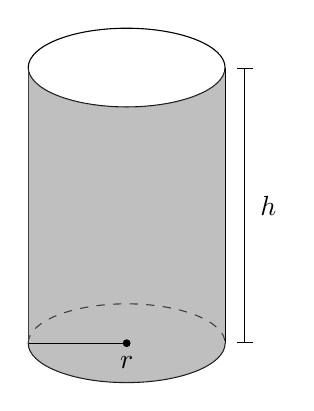
\begin{tikzpicture}
        \draw (0,0) ellipse (1.25 and 0.5);
        \draw (-1.25,0) -- (-1.25,-3.5);
        \draw (-1.25,-3.5) arc (180:360:1.25 and 0.5);
        \draw [dashed] (-1.25,-3.5) arc (180:360:1.25 and -0.5);
        \draw (1.25,-3.5) -- (1.25,0);
        \fill [gray,opacity=0.5] (-1.25,0) -- (-1.25,-3.5) arc (180:360:1.25 and 0.5) -- (1.25,0) arc (0:180:1.25 and -0.5);
        \draw (1.8,-1.75) node{$h$};
        \draw [|-|] (1.5,0) -- (1.5,-3.5);
        \draw (0,-3.75) node{$r$};
        \draw [line width=0.0mm] (-1.24,-3.5) -- (0,-3.5);
        \node at (0,-3.5) [circle,fill,inner sep=1pt]{};
    \end{tikzpicture}
\end{center}

Definimos la función de la capacidad de almacenamiento del silo como:

\begin{align*}
    V(r, h) & = \pi r^2h
\end{align*}

Por motivos estructurales, el radio no puede ser menor a 1 metro y la altura no puede superar los 24 metros. 
A su vez, 
por el material elegido, 
la altura no debe superar 3 veces al radio. 
Por lo tanto:

\begin{align*}
    3r = h
\end{align*}

Sustituimos en la expresión original:

\begin{align*}
    V & = \pi r^2 \cdot 3r \\
    V & = 3 \pi r^3
\end{align*}

Gráficamente:

\begin{center}
    \begin{tikzpicture}
        \begin{axis}[
                axis lines = left,
                xlabel = \(r\),
                ylabel = {\(V\)},
                clip = false,
                legend pos = outer north east,
                ymin = 0,
                xmin = 0,
            ]
            % volumen
            \addplot [
                domain=1:8,
                samples=200,
                color=orange,
            ]
            {3 * 3.14159265 * x * x * x};
            \addlegendentry{\(V = 3 \pi r^3\)}


        \end{axis}
    \end{tikzpicture}
\end{center}

Dadas las restricciones al radio y la altura, el dominio de la función sería $D = [1; 8]$.

Por su parte, la imagen sería $I = [9.43; 4825.49]$.

\subsection*{1.C}

La información que brinda la velocidad media en el intervalo $[1, 7]$ es insuficiente para calcular la velocidad en $t=2$, así como en $t=4$, puesto que es igual a 0. Para conocer la velocidad en esos instantes es preciso determinar la derivada de la función que, como dijimos en el apartado anterior, es $h'(t)=40-10t$. Con esta expresión es posible calcular la velocidad instantánea para todo el dominio de la función considerada.
\subsection*{Actividad 1.2}

El problema propone un cilindro con la siguiente descripción:

\begin{center}
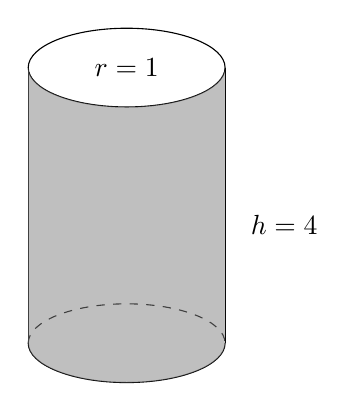
\begin{tikzpicture}
\draw (0,0) ellipse (1.25 and 0.5);
\draw (-1.25,0) -- (-1.25,-3.5);
\draw (-1.25,-3.5) arc (180:360:1.25 and 0.5);
\draw [dashed] (-1.25,-3.5) arc (180:360:1.25 and -0.5);
\draw (1.25,-3.5) -- (1.25,0);  
\fill [gray,opacity=0.5] (-1.25,0) -- (-1.25,-3.5) arc (180:360:1.25 and 0.5) -- (1.25,0) arc (0:180:1.25 and -0.5);
\draw (2,-2) node{$h = 4$};
\draw (0,0) node{$r = 1$};
\end{tikzpicture}
\end{center}

El volumen del agua en función de la altura sigue el modelo $V(h) = 4\pi h$. 

La tasa media del volumen del agua entre los puntos $[2,2.5]$ es:

\begin{align*}
    V_m &= \frac{V_{(2,5)} - V_{(2)}}{2,5-2}\\
    V_m &= \frac{4\pi\frac{5}{2} - 4\pi 2}{\frac{5}{2}-2}\\
    V_m &= 4\pi
\end{align*}

Dados dos puntos cualesquiera, $a$ y $b$, llegamos a la expresión:

\begin{align*}
    V_m &= \frac{V_{(b)} - V_{(a)}}{b-a}\\
    V_m &= \frac{4\pi b - 4\pi a}{b-a}\\
    V_m &= \frac{4\pi \cancel{(b - a)}}{\cancel{b-a}}\\
    V_m &= 4\pi
\end{align*}

Con ello podemos concluir que, a diferencia de lo que ocurría en el modelo anterior, 
en este caso la pendiente permanece constante a lo largo de la función, 
por lo cual la velocidad media es un mejor indicador del cambio en la función.
\subsection*{Actividad 1.3}

Modelos de automóvil 1 y 2.

\begin{align*}
    D_1 & = t             &
    D_2 & = \frac{t^2}{2}
\end{align*}

\subsubsection*{Parte A}

\textbf{a)} Representación gráfica de los dos modelos.

\begin{center}
    \begin{tikzpicture}
        \begin{axis}[
                axis lines = left,
                xlabel = \(t\),
                ylabel = {\(D(t)\)},
                clip = false,
            ]
            % D_1
            \addplot [
                domain=0:10,
                samples=200,
                color=blue,
            ]
            {x};
            \addlegendentry{\(D_1=t\)}

            % D_2
            \addplot[
                domain=0:10,
                samples=200,
                color=red,
            ]
            {x*x/2};
            \addlegendentry{\(D_2=\frac{t^2}{2}\)}
        \end{axis}
    \end{tikzpicture}
\end{center}

\textbf{b)} Kilómetros recorridos al cabo de 1, 2 y 3 minutos.

\begin{center}
    \begin{tabular}{ c c c }
        t      & $D_1$ & $D_2$ \\
        \hline &               \\ [-1em]
        1      & 1     & $1/2$ \\
        2      & 2     & 2     \\
        3      & 3     & $9/2$ \\
        \hline
        \vspace{12pt}
    \end{tabular}
\end{center}

\textbf{c)} Velocidad media en intervalos [0, 1], [0, 2], [0, 3] y [1, 2].

\begin{center}
    \begin{tabular}{ c c c }
        Intervalo & $D_1$ & $D_2$ \\
        \hline    &               \\ [-1em]
        $[0, 1]$  & 1     & $1/2$ \\
        $[0, 2]$  & 1     & 1     \\
        $[0, 3]$  & 1     & $3/2$ \\
        $[1, 2]$  & 1     & $3/2$ \\
        \hline
    \end{tabular}
\end{center}

\textbf{Conclusiones.}
Observando la velocidad media del modelo 1 se puede notar que esta es constante para toda la trayectoria,
situación lo esperable en un modelo lineal.
Como la pendiente es constante,
el cambio en la distancia es proporcional al cambio en el tiempo.

La situación es diferente en el modelo 2.
Al tratase de un modelo cuadrático,
la velocidad media cambia según el período de tiempo considerado,
creciendo constantemente en función del tiempo.

Ello llevaría a concluir que uno de los automóviles se desplaza de manera uniforme,
mientras el otro lo hace de manera uniformemente variada.

\vspace{10pt}

\textbf{d)} Para calcular la velocidad en los minutos 1 y 2 recurrimos a la derivada de cada una de las funciones:

\begin{align*}
    D_1' & = 1 &
    D_2' & = t
\end{align*}

\begin{center}
    \begin{tabular}{ c c c }
        t      & $D'_1$ & $D'_2$ \\
        \hline &                 \\ [-1em]
        1      & 1      & 1      \\
        2      & 1      & 2      \\
        \hline
    \end{tabular}
\end{center}

\textbf{e)} Las tangentes a la distancia recorrida por el automóvil 2, en los puntos 1 y 2, son las siguientes:

\begin{center}
    \begin{tikzpicture}
        \begin{axis}[
                axis lines = left,
                xlabel = \(t\),
                ylabel = {\(D(t)\)},
                clip = false,
            ]
            % D'_2 en 1
            \addplot [
                domain=0:10,
                samples=200,
                color=purple,
            ]
            {x-0.5};
            \addlegendentry{\(D'_{2(1)}=t-\frac{1}{2}\)}

            % D'_2 en 1
            \addplot [
                domain=0:10,
                samples=200,
                color=cyan,
            ]
            {2*x-2};
            \addlegendentry{\(D'_{2(2)}=2t-2\)}

            % D_2
            \addplot[
                domain=0:10,
                samples=200,
                color=orange,
            ]
            {x*x/2};
            \addlegendentry{\(D_2=\frac{t^2}{2}\)}
        \end{axis}
    \end{tikzpicture}
\end{center}

Las expresiones de las rectas tangentes se obtienen recurriendo a la notación punto-pendiente ($y-y_0 = m(x-x_0)$), despejando la $y$.

\vspace{10pt}

\textbf{f)} Como se desprende tanto de la tabla como de la representación gráfica, la velocidad del automóvil 1 es constante, mientras la del automóvil 2 se incrementa a medida que pasa el tiempo.

\subsubsection*{Parte B}

\begin{center}
\begin{tikzpicture}
\begin{axis}[
    axis lines = left,
    xlabel = \(t\),
    ylabel = {\(D(t)\)},
    clip = false,
]

% D_2
\addplot[
    domain=0:3,
    samples=200,
    color=cyan,
]
{x*x/2};
\addlegendentry{\(D_2=\frac{t^2}{2}\)}

% Derivada que pasa por 2
\addplot[
    domain=1:3,
    samples=200,
    color=orange,
]
{2*x-2};
\addlegendentry{\(D'_2=2t-2\)}

\node[label={270:{(2,2)}},circle,fill,inner sep=2pt] at (axis cs:2,2) {};

\end{axis}
\end{tikzpicture}
\end{center}

Para obtener la función que describe a la recta tangente a la función en el punto $(2, 2)$ expresamos este punto en la notación punto-pendiente, incluyendo como pendiente al valor devuelto por la derivada de $D_2$, que en ese punto es 2. Entonces:

\begin{align*}
    y-2 &= 2(x-2)\\
    y &= 2x - 4 + 2\\
    y &= 2x - 2
\end{align*}

Por otra parte, para obtener la función que describe la recta secante correspondiente al intervalo $[1,5; 2]$, calculamos en primer lugar su pendiente:

\begin{align*}
    m &= \frac{D_{2(2)} - D_{2(1,5)}}{2 - 1,5}\\
    m &= \frac{2 - 9/8}{2 - 1,5}\\
    m &= \frac{7}{4}
\end{align*}

Con la expresión de la pendiente, tomamos uno de los puntos por el cual deseamos que cruce, en este caso puede ser $(2, 2)$, y planteamos la función en notación punto-pendiente:

\begin{align*}
    y-2 &= \frac{7}{4}(x-2)\\
    y &= \frac{7}{4}x - \frac{7}{2} + 2\\
    y &= \frac{7}{4}x - \frac{3}{2}
\end{align*}

Con la expresión $y = \frac{7}{4}x - \frac{3}{2}$, podemos representar la secante.

\begin{center}
\begin{tikzpicture}
\begin{axis}[
    axis lines = left,
    xlabel = \(t\),
    ylabel = {\(D(t)\)},
    clip = false,
]

% D_2
\addplot[
    domain=1:3,
    samples=200,
    color=cyan,
]
{x*x/2};
\addlegendentry{\(D_2=\frac{t^2}{2}\)}

% Secante que pasa por 2
\addplot[
    domain=1.5:2,
    samples=200,
    color=magenta,
]
{7/4*x-3/2};
\addlegendentry{\(S=\frac{7}{4}t - \frac{3}{2}\)}

\node[label={270:{(2,2)}},circle,fill,inner sep=2pt] at (axis cs:2,2) {};
\node[label={270:{(1,5,9/8)}},circle,fill,inner sep=2pt] at (axis cs:1.5,1.125) {};
\end{axis}
\end{tikzpicture}
\end{center}

\begin{center}
\begin{tabular}{ c c c c c c c c c c c c }
    t & 1,5 & 1,9 & 1,99 & 1,999 & 1,9999 & 2 & 2,0001 & 2,001 & 2,01 & 2,1 & 2,5\\
	\hline \\
    $g_{(t)} = \frac{t^2}{2}$ & 1.125 & 1.805 & 1.98 & 1.998 & 1.9998 & 2 & 2.0002 & 2.002 & 2.02 & 2.205 & 3.125 \\
    \vspace{10pt} \\
    $\frac{g_(t) - g_(2)}{t - 2}$ & 1.75 & 1.95 & 2 & 2 & 2 & 2 & 2 & 2 & 2 & 2.05 & 2.25\\
    \vspace{10pt} \\
    \hline
\end{tabular}
\end{center}

Como puede observarse tanto en las gráficas como en la tabla construida, a medida que los extremos de la recta secante se aproximan, el valor de su pendiente tiende al valor de la derivada en dicho punto.

\section*{Actividad 2}

Para aproximarnos al problema de la princesa Dido desde la optimización, podemos imaginar una elipse, cuyos semiejes denominaremos $a$ y $b$.

\begin{center}
    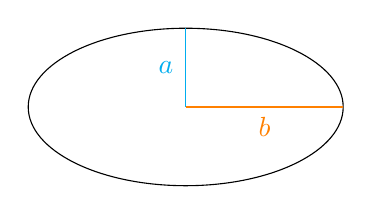
\begin{tikzpicture}
        \draw (0,0) ellipse (2cm and 1cm);
        \draw[-, cyan] (0,0) -- (0,1); % línea a
        \draw[cyan] (-0.25,0.5) node{$a$}; % label a
        \draw[-, orange] (0,0) -- (2,0); % línea b
        \draw[orange] (1,-0.25) node{$b$}; % label b
    \end{tikzpicture}
\end{center}

Podemos plantear dos ecuaciones, una para su área:

\begin{align*}
    A &= \pi ab
\end{align*}

Y otra para su perímetro:

\begin{align*}
    P &= \pi (a + b)
\end{align*}

En nuestro caso, el perímetro funciona como una restricción, a partir de la cual podemos despejar $a$, para expresar el área del elipse en función de $b$:

\begin{align*}
    \pi (a + b) &= 100\\
    a &= \frac{100}{\pi} - b
\end{align*}

Expresamos el área en función de $b$:

\begin{align*}
    A &= \pi b (\frac{100}{\pi} - b)\\
    A &= 100b - \pi b^2
\end{align*}

Derivamos esta función:

\begin{align*}
    \frac{dA}{dx} &= 100 - 2 \pi b
\end{align*}

E igualamos a 0, para determinar el punto máximo de la función del área:

\begin{align*}
    100 - 2 \pi b &= 0\\
    b &= \frac{-100}{-2 \pi}\\
    b &= \frac{50}{\pi}
\end{align*}

De ahí determinamos que $a$ es: 

\begin{align*}
    a &= \frac{100}{\pi} - \frac{50}{\pi}\\
    a &= \frac{50}{\pi}\\
    a &= b
\end{align*}

La elipse cuyos semiejes son iguales, en este caso $a$ y $b$, es el círculo. El círculo sería entonces la figura que maximizaría el área.


\subsection*{Parte B}

\subsection*{Actividad 1}

El problema pide calcular el desplazamiento y la distancia recorrida por un drone,
dada una función de su velocidad, medida en $\frac{m}{s}$. 
La velocidad del drone viene definida por la función $V_{(t)} = t^2 - t - 6$.

\begin{center}
    \begin{tikzpicture}
        \begin{axis}[
                axis lines = middle,
                xlabel = \(t\),
                ylabel = {\(V(t)\)},
                clip = false,
            ]
            % V_t
            \addplot [
                domain=0:4,
                samples=200,
                color=cyan,
            ]
            {x*x-x-6};
            \addlegendentry{\(V_{(t)} = t^2 - t - 6\)}

        \end{axis}
    \end{tikzpicture}
\end{center}

Si operamos la integral de esta función -que, al tratarse de un polinomio, se puede hacer de manera directa- obtenemos la función $d_{(t)} = \frac{t^3}{3} - \frac{t^2}{2} - 6t + C$. Notar que la primitiva de la función expresa el área bajo la curva, por lo que estaría expresada en $m$. Sería entonces una función que devolvería la distancia recorrida por el Drone.

Se nos pide considerar el desplazamiento dentro del intervalo $[1, 4]$. 
Sin embargo, en el intervalo $[1, 3]$ la integral sería negativa. 
Ello nos invita a pensar que el drone, en ese período, se desplazó en un sentido, cambiando dicho sentido en $(3, 4]$.

Entonces, podríamos pensar que el desplazamiento final del drone implicaría restar las distancias recorridas. Por su parte, obtener la distancia recorrida total implicaría sumar el módulo de ambos desplazamientos, con independencia del sentido en que el drone se haya desplazado.

Operamos la integral definida para cada uno de estos intervalos.

\begin{align*}
    \int_{1}^{3} t^2 - t - 6 \,dx             & = \frac{t^3}{3} - \frac{t^2}{2} - 6t \Big|_1^3             \\
    \frac{3^3}{3} - \frac{3^2}{2} - 6 \cdot 3 & - \left( \frac{1^3}{3} - \frac{1^2}{2} - 6 \cdot 1 \right) \\
    - \frac{22}{3}
\end{align*}

\begin{align*}
    \int_{3}^{4} t^2 - t - 6 \,dx             & = \frac{t^3}{3} - \frac{t^2}{2} - 6t \Big|_3^4             \\
    \frac{4^3}{3} - \frac{4^2}{2} - 6 \cdot 4 & - \left( \frac{3^3}{3} - \frac{3^2}{2} - 6 \cdot 3 \right) \\
    \frac{17}{6}
\end{align*}

Entonces, el desplazamiento del drone vendría dado por la expresión $\frac{17}{6} - \frac{22}{3}$, siendo $- \frac{9}{2}$. Por su parte, el recorrido total sería $|\frac{17}{6}| + |\frac{22}{3}|$, siendo $\frac{61}{6}$ el recorrido total del drone.

\end{document}
